\documentclass[]{article}

% Imported Packages
%------------------------------------------------------------------------------
\usepackage{amssymb}
\usepackage{amstext}
\usepackage{amsthm}
\usepackage{amsmath}
\usepackage{enumerate}
\usepackage{fancyhdr}
\usepackage[margin=1in]{geometry}
\usepackage{graphicx}
\usepackage{graphicx}
\graphicspath{{../signatures/}}
%\usepackage{extarrows}
%\usepackage{setspace}
%------------------------------------------------------------------------------

% Header and Footer
%------------------------------------------------------------------------------
\pagestyle{plain}  
\renewcommand\headrulewidth{0.4pt}                                      
\renewcommand\footrulewidth{0.4pt}                                    
%------------------------------------------------------------------------------

% Title Details
%------------------------------------------------------------------------------
\title{Deliverable \#2 Template}
\author{SE 3A04: Software Design II -- Large System Design}
\date{}                               
%------------------------------------------------------------------------------

% Document
%------------------------------------------------------------------------------
\begin{document}

\maketitle	
\noindent{\bf Tutorial Number:} T0x\\
{\bf Group Number:} Gx \\
{\bf Group Members:} 
\begin{itemize}
	\item List all Group Member Names (as listed in Avenue)
	\item You do not need to use student \#s or macid (keep those private).
\end{itemize}

\section*{IMPORTANT NOTES}
\begin{itemize}
	%	\item You do \underline{NOT} need to provide a text explanation of each diagram; the diagram should speak for itself
	\item Please document any non-standard notations that you may have used
	\begin{itemize}
		\item \emph{Rule of Thumb}: if you feel there is any doubt surrounding the meaning of your notations, document them
	\end{itemize}
	\item Some diagrams may be difficult to fit into one page
	\begin{itemize}
		\item Ensure that the text is readable when printed, or when viewed at 100\% on a regular laptop-sized screen.
		\item If you need to break a diagram onto multiple pages, please adopt a system of doing so and thoroughly explain how it can be reconnected from one page to the next; if you are unsure about this, please ask about it
	\end{itemize}
	\item Please submit the latest version of Deliverable 1 with Deliverable 2
	\begin{itemize}
		\item Indicate any changes you made.
	\end{itemize}
	\item If you do \underline{NOT} have a Division of Labour sheet, your deliverable will \underline{NOT} be marked
\end{itemize}

\newpage
\section{Introduction}
\label{sec:introduction}
% Begin Section

This section should provide an brief overview of the entire document.

\subsection{Purpose}
\label{sub:purpose}
% Begin SubSection
The purpose of this document is to outline the architectural framework of the Secure Chat Android Application, highlighting the principal design elements and architectural choices. Intended for a broad spectrum of internal stakeholders, including project managers, developers, domain experts, and team members, this document aims to provide a comprehensive understanding of the system’s architecture. Familiarity with the Software Requirements Specification (SRS) and a foundational technical knowledge will enhance comprehension of the details presented herein.
% End SubSection

\subsection{System Description}
\label{sub:system_description}
% Begin SubSection
The Secure Chat Android Application is designed to facilitate encrypted communication among employees of an organization holding sensitive information and trade secrets. In light of increasing threats of corporate espionage, the application incorporates a Key Distribution Centre (KDC), mediated authentication protocols, and robust symmetric-key cryptography to ensure secure message exchange. Additionally, it maintains a secure log of chat histories, thereby meeting the organization's stringent security requirements. The system's architecture is crafted to support these functionalities efficiently, ensuring both security and usability.

% End SubSection

\subsection{Overview}
\label{sub:overview}
% Begin SubSection
Following this introduction, Section 2 unveils the Analysis Class Diagram, providing insights into the application's structure through a detailed class hierarchy. Section 3 delves into the architectural design, discussing the rationale behind the chosen architecture, the interplay between subsystems, and the design considerations that underpin the application's development. Lastly, Section 4 presents Class Responsibility Collaboration (CRC) Cards, offering a deeper exploration of classes, their responsibilities, and interactions, thereby rounding off the comprehensive architectural overview of the Secure Chat Android Application.

% End SubSection

% End Section

\section{Analysis Class Diagram}
\label{sec:analysis_class_diagram}
% Begin Section
This section should provide an analysis class diagram for your application.
% End Section


\section{Architectural Design}
\label{sec:architectural_design}
% Begin Section
This section should provide an overview of the overall architectural design of your application. Your overall architecture should show the division of the system into subsystems with high cohesion and low coupling.

\subsection{System Architecture}
\subsection{System Architecture}
\label{sub:system_architecture}
% Begin SubSection
\begin{itemize}
	\item SecureChat utilizes a layered architectural approach tailored for an Android-based application, promoting modularity and scalability in its design. This architecture divides the system into three distinct layers: Presentation, Business Logic, and Data Access, each responsible for different aspects of the application's functionality.
	
	\item The architecture used is the "Layered Architecture" pattern. This pattern is specifically chosen for its provision of a clear separation of concerns among the various components of the application, which facilitates ease of maintenance and the flexibility for future development.

	\item The rationale behind choosing this architecture centers on its ability to provide a secure, robust, and adaptable foundation for the application. The separation of concerns among different system parts aids in maintenance and future expansions. This delineation between user interface, processing logic, and data management components strikes a balance between user-friendliness and strict security requirements. Furthermore, the architecture's modular nature supports the gradual integration of new features and technologies, ensuring the application's long-term adaptability without requiring significant system overhauls.
	
	\item [structural architecture diagram and its description, detailing the relationships among the subsystems.]

	\item In developing SecureChat, we explored various architectural designs before settling on our final choice. Service-Oriented Architecture (SOA), known for its discrete services and reusability, was considered but deemed too complex for our straightforward requirements. Microservices architecture, offering high scalability and flexibility, was also considered but ultimately regarded as excessive for the integrated nature of SecureChat. Event-Driven Architecture (EDA) was contemplated for its real-time responsiveness; however, its complexity in managing event queues and handlers led us to discard it. These alternatives were evaluated against our priorities of security, cohesion, and straightforward usability, guiding us towards a unified and less segmented approach to ensure SecureChat's security, performance, and maintainability.
\end{itemize}
% End SubSection


\subsection{Subsystems}
\label{sub:subsystems}
% Begin SubSection
 Provide a list of your subsystems, with a brief description of each. Be sure to document its purpose and relationship to other subsystems.

% End SubSection

% End Section
	
\section{Class Responsibility Collaboration (CRC) Cards}
\label{sec:class_responsibility_collaboration_crc_cards}
% Begin Section
This section should contain all of your CRC cards.

\begin{itemize}
	\item Provide a CRC Card for each identified class
	\item Please use the format outlined in tutorial, i.e., 
	\begin{table}[ht]
		\centering
		\begin{tabular}{|p{5cm}|p{5cm}|}
		\hline 
		 \multicolumn{2}{|l|}{\textbf{Class Name:}} \\
		\hline
		\textbf{Responsibility:} & \textbf{Collaborators:} \\
		\hline
		\vspace{1in} & \\
		\hline
		\end{tabular}
	\end{table}
	
\end{itemize}
% End Section

\appendix
\section{Division of Labour}
\label{sec:division_of_labour}
% Begin Section
Include a Division of Labour sheet which indicates the contributions of each team member. This sheet must be signed by all team members.
% End Section
\subsection{Awurama Nyarko}
\label{subsec:awurama_nyarko}
\begin{itemize}
	\item 1.1 Purpose
	\item 1.2 System Description
	\item 1.3 Overview
	\item 3.1 System Architecture: explained used of MVC and Repository
\end{itemize}
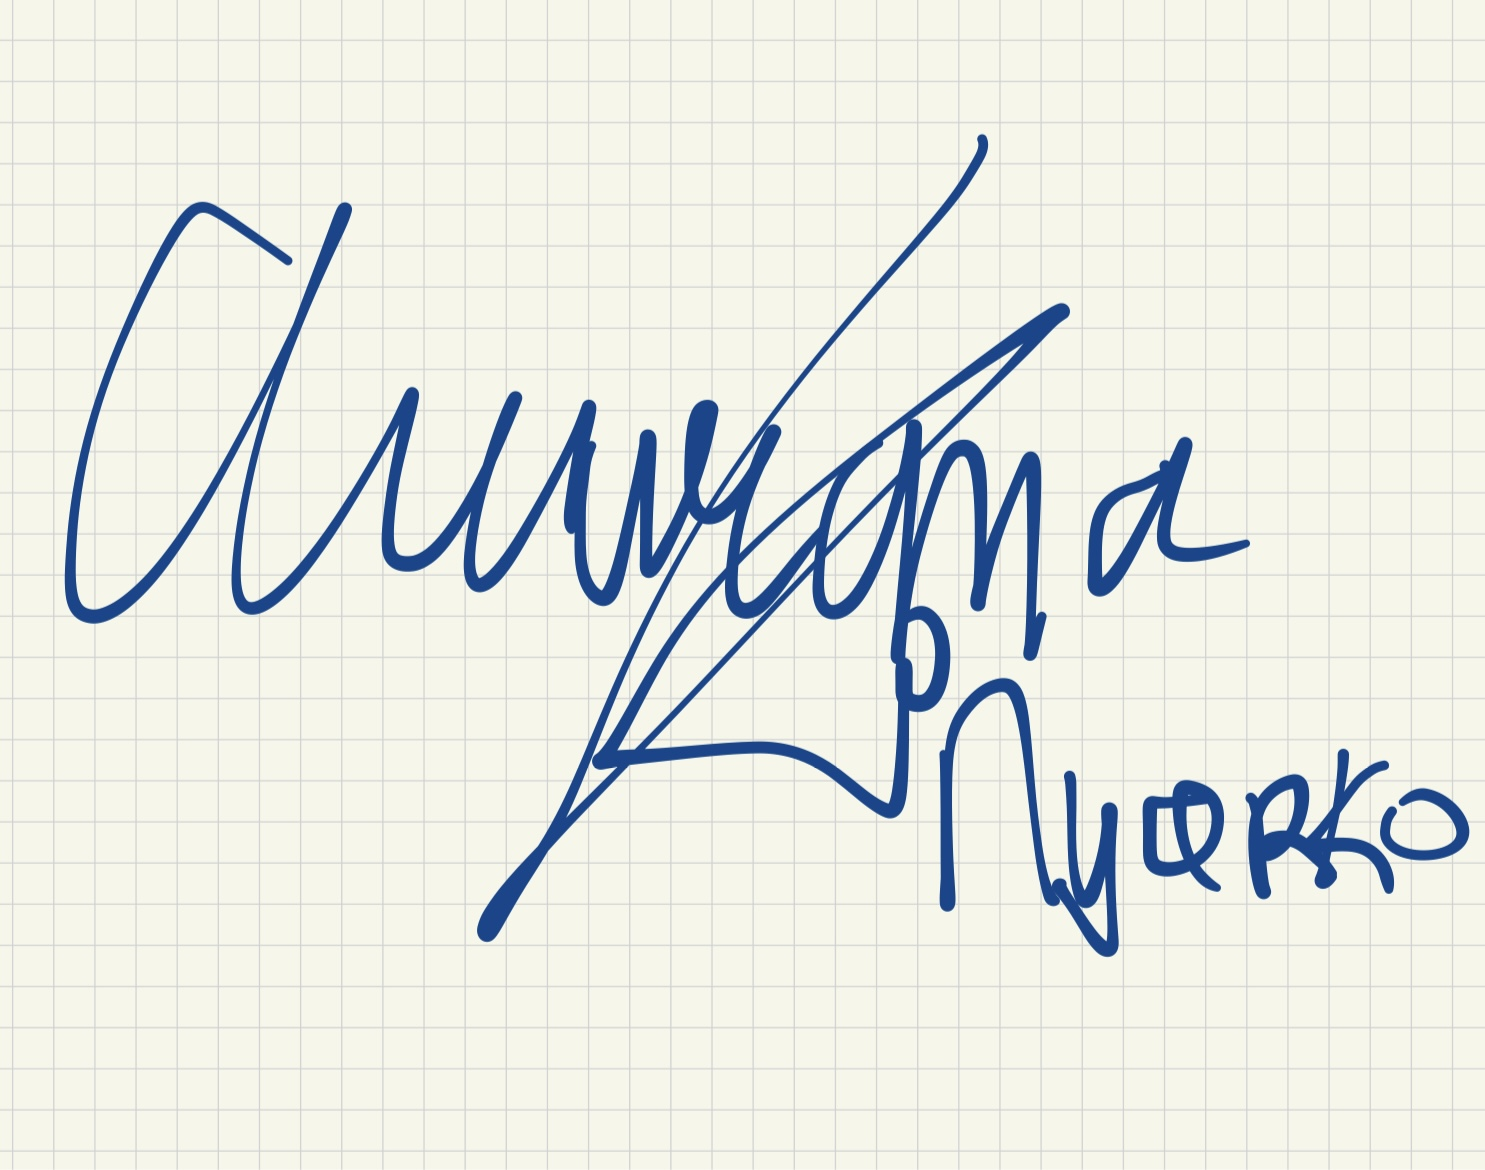
\includegraphics[width=0.5\textwidth]{awurama.jpg}

\subsection{Chelsea Maramot}
\label{subsec:chelsea_maramot}
\begin{itemize}
	\item Figure 1. Part of Analysis Class Diagram
	\item Class Responsibility Collaboration (CRC) cards
 		\begin{itemize}
   			\item File Management: File Error Handling
      			\item File Management: File Access
	 		\item File Management: File Search and Retrieval
    			\item Account Management: Account Management
       			\item Account Management: Account Database
	  		\item Account Management: User Information
     			\item Account Management: Log-in/Sign-in
			\item Account Management: Change Status
   			\item Account Management: View Account
      		\end{itemize}
\end{itemize}
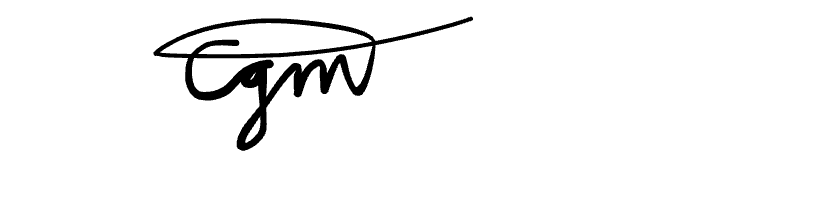
\includegraphics[width=0.5\textwidth]{chelsea.png}

\subsection{Harrison Chiu}
\label{subsec:harrison_chiu}
\begin{itemize}
	\item 3.1 System Architetcure: explained elimiation of other architecture designs
	\item Figure 2. System Architecture
 	\item 3.2 Subsystems
\end{itemize}

\includegraphics[width=0.5\textwidth]{harrison.png}

\subsection{Khushi Bhojane}
\label{subsec:khushi_bhojane}
\begin{itemize}
	\item Figure 1. Part of Analysis Class Diagram
	\item Class Responsibility Collaboration (CRC) cards
 		\begin{itemize}
   			\item Authentication Management: Encryption
      			\item Authentication Management: Token Generation
	 		\item Authentication Management: Authentication Management
    			\item Chat Management: Send Message
       			\item Chat Management: Send Files
	  		\item Chat Management: Edit/Delete Message
     			\item Chat Management: Disappearing/Vanishing Messages
			\item Chat Management: Load Previous Messages
   			\item Chat Management: 'Delivered' Status Message
      		\end{itemize}
\end{itemize}
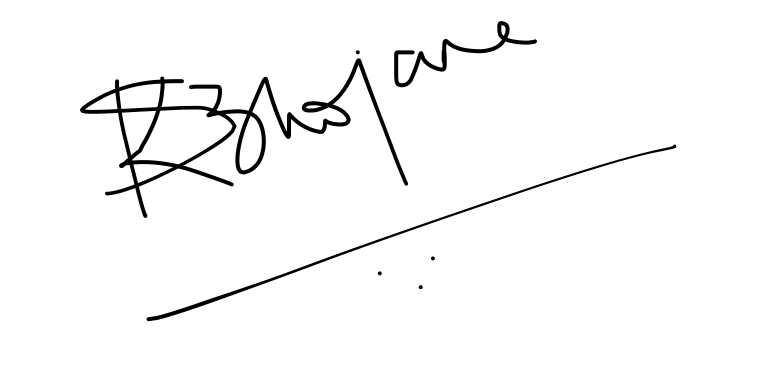
\includegraphics[width=0.5\textwidth]{khushi_signature.png}

\subsection{Sumanya Gulati}
\label{subsec:sumanya_gulati}
\begin{itemize}
	\item Figure 1. Part of Analysis Class Diagram
	\item Class Responsibility Collaboration (CRC) cards
 		\begin{itemize}
   			\item Chat Management: Chat History Database
      			\item Chat Management: Create Group
	 		\item Chat Management: Edit Group Members
    			\item Chat Management: Edit Group Details
       			\item Chat Management: Message Error
	  		\item Chat Management: Chat Management
     			\item File Management: File Management
			\item File Management: File Permissions
      		\end{itemize}
\end{itemize}

\includegraphics[width=0.5\textwidth]{signature.jpeg}

\end{document}
%------------------------------------------------------------------------------
